\section{\tool{}: Precise Side-Channel Analysis}
\label{sec:trace-qif}
In this section, we discuss how \tool{} quantifies the amount of leaked
information. We first present the limitation of existing quantification metrics.
Then, we introduce our model, the mathematical notation used in the
paper, and our method.

\subsection{Problem Setting}
Existing static side-channel quantification
works~\cite{182946,Wichelmann:2018:MFF:3274694.3274741,zhang2010sidebuster} define information
leakage using max entropy or Shannon entropy.  If zero bits of
information leakage is reported, a program is secure. However, when a tool using these metrics reports leakage, it is the ``average'' leakage. In a real attack, the leakage could be dramatically different.

 \begin{figure}[h!]
    \vspace*{-5pt}
    \centering
    \begin{lstlisting}[xleftmargin=.03\textwidth,xrightmargin=.01\textwidth]
char key[9] = input();
if(strcmp(key, "password"))   // leakage site C
    pass();                   // branch 1
else
    fail();                   // branch 2
\end{lstlisting}
\vspace*{-10pt}
    \caption{A dummy password checker}
    \label{fig:password-checker}
\vspace*{-5pt}
\end{figure}

Consider a password checker sketched in Figure~\ref{fig:password-checker}.
The password checker takes an 8-byte char array (exclude \textsf{NULL} character) 
and checks if the input is the correct password. If an attacker uses a side-channel attack to determine that the code executes branch
$\{{1\}}$, they can infer the password equals to
``password'', in which case the attacker retrieves the full password.
Therefore, the total leaked information should be 64 bits, which equals to the
size of the original sensitive input when the code executes branch
$1$.

However, prior static approaches cannot precisely capture the amount of leakage. According to the definition of Shannon entropy, the leakage will be
$\frac{1}{2^{64}}*\log_{2}\frac{1}{2^{64}} + \frac{2^{64}-1}{2^{64}}
*\log_{2}\frac{2^{64}-1}{2^{64}} \approx 0$ bits. Max-entropy is defined from the
number of possible observations. Because the program has two
branches, tools based on max-entropy will report the code has a $\log_2{2} = 1$
bit leakage.

\begin{figure}[h]
    \vspace*{-5pt}
    \centering
    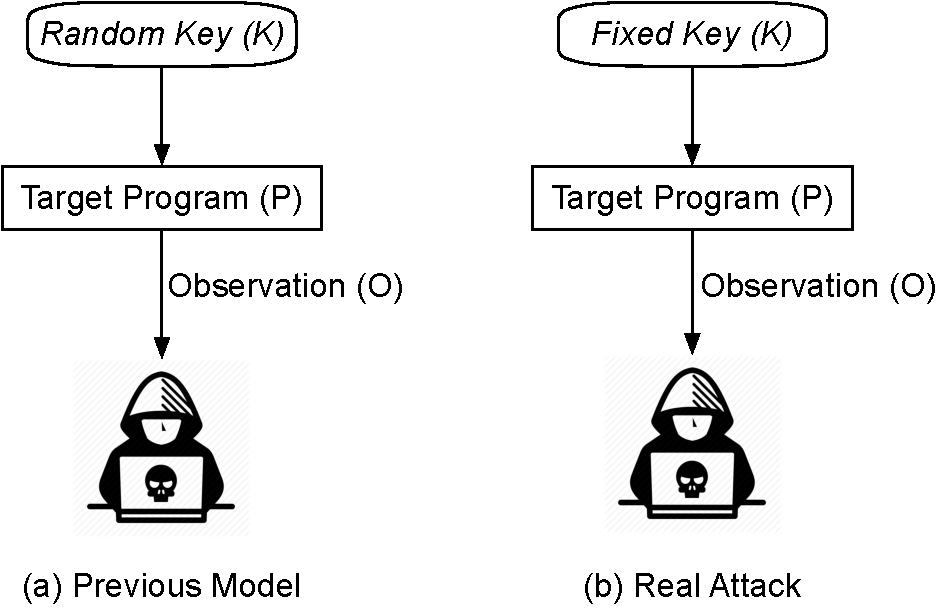
\includegraphics[width=.65\columnwidth]{./figures/RA.pdf}
\vspace*{-2pt}
    \caption{The gap between a real attack and previous models}\label{fig:gap}
    \vspace*{-5pt}
\end{figure}

Both approaches fail to tell how much information is leaked an actual execution. 
The problem~\cite{Chattopadhyay:2017:QIL:3127041.3127044} with existing methods is that their approaches do not consider input values and 
real runtime information. 
They assume an attacker runs the program multiple times with many different or 
random sensitive inputs. As
shown in Figure~\ref{fig:gap}\,(a), both Shannon entropy and max-entropy
give an ``average'' estimate of the information leakage. However, generating random inputs is
not the typical scenario for an adversary launching a side-channel attack. In
a typical attack, the adversary wants to retrieve sensitive
information, which is typically fixed (e.g., AES keys).
The adversary performs their attack over and over again with fixed input and 
guess the value bit by
bit (e.g., Kocher's timing attacks~\cite{kocher1996timing}), as in Figure~\ref{fig:gap}\,(b). 
We need a theory for dynamic analysis that says an attack leaks $x$ bits of
secret information, where $x$ is useful in estimating the sensitive level of the vulnerability. 
However, all previous methods fail for real attack models. This is the first challenge we face
\textbf{(Challenge C1)}.
\jl{Tis explaination of why previous techniques fail should also be in the introduction.}

\subsection{Notation}
In the section, we give necessary definitions and notation for dealing with
programs and side-channels. We use capital letters (e.g., $A$) to represent a
set. $|A|$ represents the cardinality of set $A$. We use corresponding lower case
letters to represent one element of the set (e.g., $a \in A$).

We assume a program ($\beta$) has $K$ as its sensitive input. $K$ should be 
a finite set of keys. The program also takes known messages $M$ as its input. 
During an AES encryption, for example, 
$\beta$ is the encryption function. $K$ is the set of all possible AES keys, 
and $M$ represents the set consisting of all plaintext messages to be encrypted. In a real execution, an adversary may have 
some observations ($O$) of the program. Examples of those observations include 
timing, CPU usages, and electromagnetic signals (EM). This paper only
uses secret-dependent control flows and secret-dependent data 
accesses as observations.

With the above definition, we have the following mapping between $\beta$,
$K$, $M$, and $O$:
%\vspace*{-0pt}
\begin{displaymath}
    \beta(K, M) \rightarrow O
\end{displaymath}


We model a side-channel in the following way. An adversary does not have
access to $K$, but he knows $\beta$, $M$, and $O$. For one execution of a
deterministic program, once $k \in K$ and $m \in M$ are fixed, the observation
($o \in O$) should also be determined. An attacker knows $\beta$, $o$,
and $m$. The attacker wants to infer the value of $k$. We use $K^o$ to denote
the set of possible $k$ values that produce the same observation: $K^o = \{ k \in K \, |\, \beta(k, m) \rightarrow o\}$

Then the problem of quantifying the amount of leaked information can be
restated as the following question:

\emph{How much uncertainty of $K$ is reduced if an attacker knows $\beta$, $m$, and $o$?}

\subsection{Theoretical Analysis \textbf{(Solution to Challenge C1)}}
In information theory, the mutual information ($I$) is a measure of the mutual
dependence between two variables. We use $I$ to describe the
dependence between original sensitive keys ($K$) and attackers' observations ($O$), which is defined as:

\begin{equation} \label{eq:1}
    I(K;O) = \sum_{k {\in} K}{\sum_{o {\in} O}{p(k, o)\log_2\frac{p(k, o)}{p(k)p(o)}}}
\end{equation}

where $p(k, o)$ is the joint probability mass function of $K$ and $O$.
Alternatively, the mutual information can also be equivalently expressed as:
\begin{equation} \label{eq:2}
    I(K;O) = H(K) - H(K|O)
\end{equation}

$H(K|O)$ is the entropy of $K$ under the condition $O$. It quantifies the
uncertainty of $K$, given the value of $O$. In other words, the conditional 
entropy $H(K|O)$ marks the uncertainty about $K$ after an adversary has 
made observations $O$.

\begin{equation}
    H(K|O) = - \sum_{o {\in} O} {p(o) \sum_{k {\in} K}{p(k|o)\log_2p(k|o)}}
\end{equation}

In this project, we hope for a very precise definition of information
leakages. Suppose an attacker runs the target program with one
input, we want to know how much information they can infer by observing the
memory access patterns ($o$). We come to the simple formulation~\cite{10.1007/978-3-642-00596-1_21,AskarovC12} %% where the information
%% leakage equals:
%% \textbf{Initial uncertainty - remaining uncertainty}
that
\begin{align*}
     & \mathit{Information\ leakage} =                                         \\
     & ~~~~ \mathit{Initial\ uncertainty} - \mathit{Remaining\ uncertainty}.
\end{align*}

Next, we compare the Eq.~(\ref{eq:2}) with the above formulation, we find $H(K)$
is the $\mathit{Initial\ uncertainty}$ and $H(K|O)$ is $\mathit{Remaining\
uncertainty}$. During a real attack, the observation ($o$) is known. Thus we
have $H(K|O) = H(K|o)$. Therefore, we define the amount of leaked information as

\begin{displaymath}
    Leakage = H(K) - H(K|o)
\end{displaymath}

For a program ($\beta$) without any domain information, all possible sensitive
inputs appear equally likely. Therefore, for any $k \in K$, $p(k) =
\frac{1}{|K|}$. We have
%\vspace*{-5pt}
$$H(K) = \sum_{k {\in} K}\frac{1}{|K|}\log_2{|K|} = \log_2{|K|}$$
%\vspace*{-5pt}

For any $k' \in K \setminus K^o$, $p(k'|o) = 0$. We get
\begin{align*}
    H(K;o) & = - \sum_{k {\in} K^o}{p(k|o)\log_2p(k|o)}                         \\
           & \qquad   - \sum_{k` {\in} (K \setminus K^o)}{p(k'|o)\log_2p(k'|o)} \\
           & = \sum_{k {\in} K^o}\frac{1}{|K^o|}\log_2{|K^o|}                   \\
           & = \log_2{|K^o|}
\end{align*}

\begin{mydef}
    \label{def}
    Given a program $\beta$ with the input set $K$,
    an adversary has the observation $o$ when the input $k{\in}K^o$.
    We denote it as
    $$\beta(K^o, m) \rightarrow	o$$

    The amount of leaked information $L_{\beta(k)\rightarrow o}$ based on the observation ($o$) is
    $$L_{\beta(k)\rightarrow o} = \log_2{|K|} - \log_2{|K^o|}$$
\end{mydef}
\vspace*{-5pt}

The above definition can be understood in an intuitive way. Suppose an attacker
guesses a 128-bit encryption key. 
Without any domain knowledge, 
they can find the key by performing an exhaustive search over $2^{128}$ possible keys. 
However, assume the program has a side-channel leakage site. After the program finishes execution, the
attacker has some observations and only needs to find the key by performing an
exhaustive search over $2^{120}$ possible keys. Then, we say that 8 bits of the information
is leaked. In this example, $2^{128}$ is the size of $K$ and $2^{120}$ is the size of $K^o$.

With this definition, if an attacker observes that the code in
Figure~\ref{fig:password-checker} executes branch 1, then $K^{o^{1}} =
\{\mathrm{``password"}\}$. Therefore, the information leakage $L_{P(k)=o^{1}} =
\log_2{2^{64}} - \log_2{1} = 64$ bits, which means the key is entirely leaked. If
the attacker observes the code hits branch 2, the leaked information is
$L_{P(k)=o^{2}} = \log_2{2^{64}} - \log_2{(2^{64}-1)} \approx 0$ bits.

As the size of input-sensitive information is
usually public, the problem of quantifying the leaked information is equivalent to the problem of estimating the size of input key $|K^o|$ under
the condition $o \in O$. 

\subsection{Our Conceptual Framework}
\label{side-channel:condition}
We now discuss how to model observations ($O$), which are the direct information
that an adversary can obtain during a side-channel attack.

During an execution, a program ($\beta$) has many temporary values ($t_i \in
T$). Once $\beta$ (program), $k$ (secret), and $m$ (message, public) are
determined, $t_i$ is also fixed (for deterministic programs). Therefore, $ t_i = f_i(\beta, k, m)$, where $f_i$ is a function that maps between $t_i$ and ($\beta$, $k$, $m$).

In the paper, we consider two code patterns that can be exploited to infer sensitive information
 by an attacker,
\emph{secret-dependent control transfers} and \emph{secret-dependent data
accesses}. 
%In other words, an adversary has observations based on control-flows and data accesses.

\subsubsection{Secret-dependent Control Transfers}
A control-flow path is secret-dependent if different input-sensitive keys
($K$) can lead to different branch conditions. 
We define a branch to be secret-dependent if:
$$\exists k_{i1}, k_{i2} \in K, \,f_i(\beta, k_{i1}, m) \neq f_i(\beta, k_{i2}, m)$$

An adversary can observe which branch the code executes if the branch condition
equals $t_b$. We use the constraint $c_i : f_i(\beta, k, m) = t_b$ to model
the observation ($o$) on secret-dependent control-transfers.

\subsubsection{Secret-dependent Data Accesses}
Similar to secret-dependent control-flow transfers, a data access operation is
secret-dependent if different input sensitive keys ($K$) cause access to different
memory addresses. We use the model from CacheD~\cite{203878}. The low $L$ bits
of the address are generally unimportant in side-channels.

A data access is secret-dependent if:
$$\exists k_{i1}, k_{i2} \in K, \,f_i(\beta, k_{i1}, m) >> L \neq f_i(\beta, k_{i2}, m) >> L$$

If the memory access equals to $t_b$, we can use the constraint $c_i :
f_i(\beta, k, m) >> L = t_b >> L$ to model the observation of a secret-dependent
data access.

%With the above definitions, we can model an attacker's observation by a series of math
%formulas. For example, in Figure~\ref{fig:side-channel}, if an attacker observes
%the code executes the branch 1, we have $c_5: k_1 + k_2 < 4$ to describe an
%attacker's knowledge and $K^{o5} = \{k_1,\, k_2\,|\, (k_1 + k_2) < 4\}$. If an
%attacker observes the code executes the branch 2, we have $c_8: k_1 - k_2 > 0$
%and $K^{o8} = \{k_1,\, k_2\,|\, (k_1 - k_2) > 0\}$.
